\documentclass[aspectratio=169]{beamer}

%% ─── Theme (Bruno: navy/red, Fira Sans, gray footer) ────────────────────────
\usetheme{Bruno}
\setbeamerfont{frametitle}{size=\normalsize, series=\bfseries}

%% footer with the real total (the theme hard-codes /25)
\makeatletter
\setbeamertemplate{footline}{%
  \leavevmode\usebeamerfont{footline}%
  \hbox{%
    \begin{beamercolorbox}[wd=.65\textwidth, ht=3ex, dp=1.25ex, left, leftskip=2em]{footline}%
      \insertshorttitle%
    \end{beamercolorbox}%
    \begin{beamercolorbox}[wd=.35\textwidth, ht=3ex, dp=1.25ex, right, rightskip=4em]{footline}%
      \insertshortauthor\hspace{1em}\insertframenumber\,/\,\inserttotalframenumber
    \end{beamercolorbox}}}
\makeatother

%% ─── Packages ────────────────────────────────────────────────────────────────
\usepackage{pifont}
\usepackage{fontawesome5}
\usepackage{xcolor}
\usepackage{tikz}
\usetikzlibrary{arrows.meta, positioning, calc, shadows, shapes.callouts, overlay-beamer-styles, fit, patterns, fadings, shapes.geometric}
\usepackage{booktabs}
\usepackage{colortbl}
\usepackage{tabularx}
\usepackage{pgfplots}
\pgfplotsset{compat=1.18}
%% legend marker: a small filled rectangle in the series colour
\pgfplotsset{box legend/.style={legend image code/.code={\fill[##1, draw=none] (0cm,-0.07cm) rectangle (0.28cm,0.11cm);}}}
\usepgfplotslibrary{groupplots}
\usepackage{numprint}
\npthousandsep{,}
\usepackage{graphicx}
\usepackage{amsmath}
\usepackage{hyperref}

%% ─── Colors (deck palette + University of Waterloo) ─────────────────────────
\definecolor{tug}{RGB}{196,13,30}
\definecolor{tugb}{RGB}{60,100,200}
\definecolor{darkgreen}{RGB}{0,130,0}
\definecolor{mygreen}{RGB}{220,245,215}
\definecolor{myorange}{RGB}{255,230,210}
\definecolor{color4}{RGB}{255,165,0}
\definecolor{uwgold}{HTML}{FED34C}
\definecolor{uwgoldD}{HTML}{EAAB00}
\definecolor{uwmath}{HTML}{A2006E}
\definecolor{uwsci}{HTML}{003599}
\definecolor{uwhealth}{HTML}{115E6B}
\definecolor{uweng}{HTML}{5D0096}
\definecolor{uwarts}{HTML}{D93F00}
\definecolor{uwgreyA}{HTML}{DFDFDF}
\definecolor{uwgreyC}{HTML}{787878}

%% ─── Blocks ──────────────────────────────────────────────────────────────────
\setbeamercolor{block title example}{bg=darkgreen, fg=white}
\setbeamercolor{block body example}{bg=mygreen, fg=black}
\setbeamercolor{block title alerted}{bg=orange!80!black, fg=white}
\setbeamercolor{block body alerted}{bg=myorange, fg=black}

%% ─── Helpers ─────────────────────────────────────────────────────────────────
\newcommand{\hred}[1]{\textcolor{tug}{\textbf{#1}}}
\newcommand{\hgreen}[1]{\textcolor{darkgreen}{\textbf{#1}}}
\newcommand{\hblue}[1]{\textcolor{tugb}{\textbf{#1}}}
\newcommand{\hring}[1]{\textcolor{uwmath}{\textbf{#1}}}
%% numbered reference marker; numbers match the References slide
\newcommand{\rf}[1]{\textsuperscript{\textcolor{gray}{\,[#1]}}}
%% #1 accent, #2 section, #3 title
\newcommand{\apptitle}[3]{\textcolor{#1}{#2}~\textcolor{black!30}{\textbar}~#3}
%% evidence tag shown under a claim
\newcommand{\evidence}[1]{{\scriptsize\textcolor{tugb}{\faSearch~\textbf{Evidence:}}~#1}}
%% section divider in the style of the defense deck
\newcommand{\sectionslide}[2]{%
\begin{frame}[plain,noframenumbering]
\begin{tikzpicture}[remember picture, overlay]
  \begin{scope}
    \clip (current page.south west) rectangle (current page.north east);
    \fill[black!58] ($(current page.north east)+(-22mm, 8mm)$) circle (48mm);
    \fill[#1]       ($(current page.north west)+( 24mm,-19mm)$) circle (13mm);
    \fill[uwgold]   ($(current page.north west)+( 51mm,-26mm)$) circle (8mm);
    \fill[gray!60]  ($(current page.north west)+( 69mm,-19mm)$) circle (2.5mm);
  \end{scope}
  \node[inner sep=0, text=#1, font=\Huge\bfseries] (st) at (current page.center) {#2};
  \draw[#1, line width=0.8pt] ([yshift=-5mm]st.south west) -- ([yshift=-5mm]st.south east);
\end{tikzpicture}
\end{frame}}

%% table icon used in the visuals
\tikzset{
  %% catalog-explorer style table: outline grid with a shaded header row
  pics/tbl/.style={code={
    \fill[white] (-5pt,-4pt) rectangle (5pt,4pt);
    \fill[#1!18] (-5pt,1.6pt) rectangle (5pt,4pt);
    \draw[#1, line width=0.4pt] (-5pt,1.6pt) -- (5pt,1.6pt);
    \draw[#1, line width=0.3pt] (-5pt,-1.2pt) -- (5pt,-1.2pt);
    \draw[#1, line width=0.3pt] (-1.6pt,-4pt) -- (-1.6pt,1.6pt) (1.7pt,-4pt) -- (1.7pt,1.6pt);
    \draw[#1, line width=0.55pt, rounded corners=0.6pt] (-5pt,-4pt) rectangle (5pt,4pt);}},
  pics/tbl/.default=tugb,
  %% catalog-explorer style catalog
  pics/cat/.style={code={
    \fill[#1!12] (-4pt,-4pt) rectangle (4pt,4pt);
    \draw[#1, line width=0.5pt, rounded corners=0.9pt] (-4pt,-4pt) rectangle (4pt,4pt);
    \fill[#1] (-2.3pt,0.7pt) rectangle (2.3pt,2.3pt);
    \draw[#1, line width=0.4pt] (-2.3pt,-1pt) -- (2.3pt,-1pt) (-2.3pt,-2.5pt) -- (2.3pt,-2.5pt);}},
  pics/cat/.default=tugb,
  %% slide 2: business and concept-table boxes
  biz/.style={draw=#1, fill=#1!4, rounded corners=3pt, line width=0.7pt, minimum width=4.2cm, minimum height=2.45cm},
  concept/.style={draw=#1!70, fill=white, rounded corners=2pt, densely dashed, line width=0.5pt, minimum width=1.45cm, minimum height=1.45cm},
}

\setlength{\itemsep}{1pt}
\setlength{\parskip}{0pt}

%% ─── Metadata ────────────────────────────────────────────────────────────────
\title[Scalable Join Discovery with LLMs and Recall Guarantees]{Scalable Join Discovery with LLMs\\ and Recall Guarantees}
\author{Saeed Fathollahzadeh}
\institute{University of Waterloo --- Data Intelligence Lab}
\date{}

%%%%%%%%%%%%%%%%%%%%%%%%%%%%%%%%%%%%%%%%%%%%%%%%%%%%%%%%%%%%%%%%%%%%%%%%%%%
\begin{document}
%%%%%%%%%%%%%%%%%%%%%%%%%%%%%%%%%%%%%%%%%%%%%%%%%%%%%%%%%%%%%%%%%%%%%%%%%%%

%% ─── TITLE ───────────────────────────────────────────────────────────────────
\begin{frame}[plain,noframenumbering]
\begin{tikzpicture}[remember picture, overlay]
  \node[align=center, text=tug, font=\LARGE\bfseries] (t) at ($(current page.center)+(0,6mm)$)
    {Scalable Join Discovery with LLMs\\[2pt] and Recall Guarantees};
  \draw[tug, line width=0.8pt] ([yshift=-3mm]t.south west) -- ([yshift=-3mm]t.south east);
  \node[align=center, font=\normalsize, text=black!80] at ($(t.south)+(0,-12mm)$)
    {Saeed Fathollahzadeh\\[2pt]{\small University of Waterloo --- Data Intelligence Lab}};
\end{tikzpicture}
\end{frame}

%% ─── OUTLINE ─────────────────────────────────────────────────────────────────
%% outline hidden for now
\iffalse
\begin{frame}{\apptitle{black!60}{Overview}{Outline}}
\vspace{4mm}
\begin{columns}[T]
\begin{column}{0.48\textwidth}
\begin{enumerate}\setlength\itemsep{7pt}
  \item \textbf{Context} --- why enterprise data needs a join graph
  \item \textbf{Evidence} --- what LLM-built join graphs look like today
  \item \textbf{Problems} --- cost, wrong joins, redundancy, inconsistency
  \item \textbf{Existing work} --- non-LLM, LLM, and hybrid methods
\end{enumerate}
\end{column}
\begin{column}{0.48\textwidth}
\begin{enumerate}\setcounter{enumi}{4}\setlength\itemsep{7pt}
  \item \textbf{Research problem} --- cost-bounded join discovery
  \item \textbf{Key insight} --- key domains, not table pairs
  \item \textbf{Our approach} --- architecture
  \item \textbf{Research questions} and evaluation plan
\end{enumerate}
\end{column}
\end{columns}
\end{frame}
\fi

%%%%%%%%%%%%%%%%%%%%%%%%%%%%%%%%%%%%%%%%%%%%%%%%%%%%%%%%%%%%%%%%%%%%%%%%%%%
% \sectionslide{tugb}{CONTEXT}  % removed
%%%%%%%%%%%%%%%%%%%%%%%%%%%%%%%%%%%%%%%%%%%%%%%%%%%%%%%%%%%%%%%%%%%%%%%%%%%

%% ─── WHY A JOIN GRAPH ────────────────────────────────────────────────────────
\begin{frame}{\apptitle{tugb}{Context}{Enterprise Data Needs a Join Graph}}
\footnotesize
\begin{columns}[T]
\begin{column}{0.44\textwidth}
\vspace{1mm}
\textbf{\hblue{The setting}}
\begin{itemize}\setlength\itemsep{2pt}
  \item Many businesses, each with \textbf{50 to 8K tables}
  \item Staging copies, snapshots, ERP exports
  \item Foreign keys are \hred{rarely declared}
\end{itemize}
\vspace{2mm}
\textbf{\hblue{Before joining: concept tables}}
\begin{itemize}\setlength\itemsep{2pt}
  \item Tag the columns of every table
  \item Build \textbf{concept tables}: cluster similar or overlapping tables
  \item Discover joins between concepts, \textbf{inside a business} and \textbf{across businesses}
\end{itemize}
\end{column}
\begin{column}{0.54\textwidth}
\centering
\resizebox{\linewidth}{!}{%
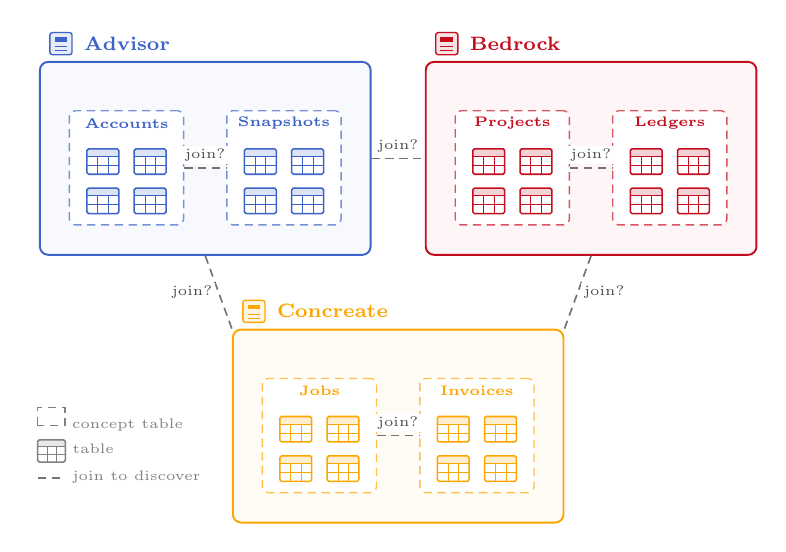
\begin{tikzpicture}[font=\scriptsize,
  jn/.style={black!55, densely dashed, line width=0.6pt},
  jlbl/.style={font=\tiny, text=black!70, fill=white, inner sep=1pt}]
  %% each business: catalog header, two concept tables, each a cluster of tables
  \foreach \cx/\cy/\col/\nm/\bn/\ca/\cb in {0/0/tugb/A/Advisor/Accounts/Snapshots, 4.9/0/tug/B/Bedrock/Projects/Ledgers, 2.45/-3.4/color4/C/Concreate/Jobs/Invoices} {
    \node[biz=\col] (b\nm) at (\cx,\cy) {};
    \pic at ($(b\nm.north west)+(0.28,0.22)$) {cat=\col};
    \node[anchor=west, font=\scriptsize\bfseries, text=\col] at ($(b\nm.north west)+(0.45,0.22)$) {\bn};
    \node[concept=\col] (c\nm1) at (\cx-1.0,\cy-0.12) {};
    \node[concept=\col] (c\nm2) at (\cx+1.0,\cy-0.12) {};
    \node[font=\tiny\bfseries, text=\col] at ($(c\nm1.north)+(0,-0.17)$) {\ca};
    \node[font=\tiny\bfseries, text=\col] at ($(c\nm2.north)+(0,-0.17)$) {\cb};
    \foreach \k in {1,2} {
      \foreach \dx/\dy in {-0.3/0.08, 0.3/0.08, -0.3/-0.42, 0.3/-0.42} {
        \pic[scale=1.15] at ($(c\nm\k)+(\dx,\dy)$) {tbl=\col};
      }
    }
    %% join inside one business
    \draw[jn] (c\nm1.east) -- node[jlbl, above=1pt] {join?} (c\nm2.west);
  }
  %% joins across businesses
  \draw[jn] (bA.east) -- node[jlbl, above=1pt] {join?} (bB.west);
  \draw[jn] (bA.south) -- node[jlbl, left=1pt] {join?} (bC.north west);
  \draw[jn] (bB.south) -- node[jlbl, right=1pt] {join?} (bC.north east);
  %% legend
  \node[anchor=north west, align=left, text=gray, font=\tiny] at ($(bC.south west)+(-2.6,1.6)$)
    {\tikz[baseline=-0.5ex]\draw[densely dashed, gray] (0,0) rectangle (0.35,0.22);\ concept table\\[2pt]
     \tikz[baseline=-0.5ex]\pic{tbl=gray};\ table\\[2pt]
     \tikz[baseline=-0.5ex]\draw[black!55, densely dashed, line width=0.6pt] (0,0) -- (0.35,0);\ join to discover};
\end{tikzpicture}}
\vspace{2mm}
\begin{exampleblock}{}
\centering\vspace{0.5mm}
\textbf{Join graph} = which tables join, \textbf{on which key}, \textbf{in which direction}
\vspace{0.5mm}
\end{exampleblock}
\end{column}
\end{columns}
\end{frame}

%% ─── CURRENT PIPELINE ────────────────────────────────────────────────────────
\begin{frame}{\apptitle{tugb}{Context}{How Join Graphs Are Built Today --- Three LLM Steps}}
\footnotesize
\vspace{3mm}
\centering
\begin{tikzpicture}[
  pstep/.style={draw=tugb, fill=white, rounded corners=3pt, line width=0.8pt, minimum width=3.6cm, minimum height=1.55cm, align=center},
  bad/.style={draw=tug, fill=tug!5},
  flow/.style={-{Latex[length=5pt,width=4pt]}, line width=1pt, black!55},
  cost/.style={font=\scriptsize, align=center}]
  \node[pstep] (s1) at (0,0) {\faTags\\[2pt]\textbf{1. Annotate tables}\\{\scriptsize tag columns, describe tables}};
  \node[pstep] (s2) at (4.6,0) {\faLayerGroup\\[2pt]\textbf{2. Cluster into concepts}\\{\scriptsize group related tables}};
  \node[pstep, bad] (s3) at (9.2,0) {\faProjectDiagram\\[2pt]\textbf{3. Pairwise join discovery}\\{\scriptsize prompt every pair: join? key?}};
  \draw[flow] (s1) -- (s2);
  \draw[flow] (s2) -- (s3);
  \node[cost, text=darkgreen] at ($(s1.south)+(0,-4mm)$) {\faCheck\ one call per table: $O(n)$};
  \node[cost, text=darkgreen] at ($(s2.south)+(0,-4mm)$) {\faCheck\ one call per batch: $O(n)$};
  \node[cost, text=tug]       at ($(s3.south)+(0,-4mm)$) {\faExclamationTriangle\ one call per pair: $O(n^2)$};
\end{tikzpicture}

\vspace{6mm}
\begin{columns}[T]
\begin{column}{0.44\textwidth}
\textbf{\hgreen{What works}}
\begin{itemize}\setlength\itemsep{3pt}
  \item The LLM reads names, descriptions, and values together
  \item It recognizes business entities that statistics miss
\end{itemize}
\end{column}
\begin{column}{0.48\textwidth}
\textbf{\hred{What breaks}}
\begin{itemize}\setlength\itemsep{3pt}
  \item Step 3 dominates cost and time
  \item Its output graph is \textbf{dense}, \textbf{redundant}, and hard to trust
\end{itemize}
\end{column}
\end{columns}
\end{frame}

%%%%%%%%%%%%%%%%%%%%%%%%%%%%%%%%%%%%%%%%%%%%%%%%%%%%%%%%%%%%%%%%%%%%%%%%%%%
%%%%%%%%%%%%%%%%%%%%%%%%%%%%%%%%%%%%%%%%%%%%%%%%%%%%%%%%%%%%%%%%%%%%%%%%%%%

%% ─── DEGREE DISTRIBUTION ─────────────────────────────────────────────────────
\begin{frame}{\apptitle{tugb}{Evidence}{LLM-built Join Graphs Are Dense}}
\footnotesize
\begin{columns}[T]
\begin{column}{0.60\textwidth}
\centering
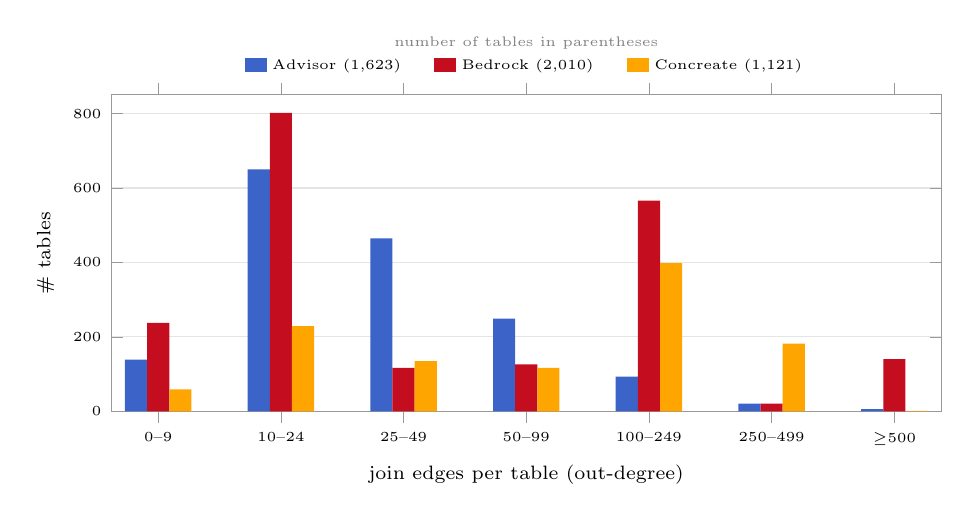
\begin{tikzpicture}
\begin{axis}[
  ybar=0pt, bar width=8pt, width=\linewidth, height=5.6cm, scale only axis=false,
  ymin=0, ymax=850, ylabel={\# tables}, ylabel style={font=\scriptsize},
  xlabel={join edges per table (out-degree)}, xlabel style={font=\scriptsize},
  title={\tiny\textcolor{gray}{number of tables in parentheses}}, title style={yshift=7pt},
  symbolic x coords={0--9,10--24,25--49,50--99,100--249,250--499,$\geq$500},
  xtick=data, x tick label style={font=\tiny, rotate=0},
  y tick label style={font=\tiny},
  box legend, legend columns=-1,
  legend style={font=\tiny, at={(0.5,1.03)}, anchor=south, draw=none, fill=none,
    /tikz/every even column/.append style={column sep=10pt}},
  legend cell align=left, enlarge x limits={abs=17pt},
  axis line style={black!40}, tick style={black!40}, ymajorgrids, grid style={black!10}]
  \addplot[fill=tugb, draw=none] coordinates {(0--9,139) (10--24,650) (25--49,465) (50--99,249) (100--249,93) (250--499,21) ($\geq$500,6)};
  \addplot[fill=tug, draw=none] coordinates {(0--9,238) (10--24,802) (25--49,117) (50--99,126) (100--249,566) (250--499,21) ($\geq$500,140)};
  \addplot[fill=color4, draw=none] coordinates {(0--9,59) (10--24,229) (25--49,135) (50--99,117) (100--249,398) (250--499,182) ($\geq$500,1)};
  \legend{{Advisor (1,623)}, {Bedrock (2,010)}, {Concreate (1,121)}}
\end{axis}
\end{tikzpicture}
\end{column}
\begin{column}{0.38\textwidth}
\vspace{3mm}
\begin{itemize}\setlength\itemsep{6pt}
  \item \textbf{Bedrock}: \hred{36\%} of tables have \textbf{$\geq$100} join edges; \textbf{140} tables have $\geq$500
  \item \textbf{Concreate}: median table has \hred{121} join edges
  \item Max: one table joins \hred{1,450} others
\end{itemize}
\vspace{3mm}
\begin{alertblock}{}
\vspace{0.5mm}
Real schemas have a handful of foreign keys per table --- not hundreds.
\vspace{0.5mm}
\end{alertblock}
\vspace{1mm}
{\tiny\textcolor{gray}{Source: exported join graphs of three businesses (top 5,000 nodes each).}}
\end{column}
\end{columns}
\end{frame}

%% ─── RED FLAGS ───────────────────────────────────────────────────────────────
%% hidden for now
\iffalse
\begin{frame}{\apptitle{tugb}{Evidence}{Red Flags in the Graph}}
\footnotesize
\vspace{2mm}
\begin{columns}[T]
\begin{column}{0.32\textwidth}
\begin{block}{\faHashtag~Generic columns as hubs}
\vspace{1mm}
Columns literally named \texttt{DATA} are linked to
\hred{1,826}, \hred{915}, and \hred{636} other columns.\\[3pt]
\textcolor{gray}{A column that ``joins'' with everything is not a key.}
\vspace{1mm}
\end{block}
\end{column}
\begin{column}{0.32\textwidth}
\begin{block}{\faCopy~Snapshots joined, not unioned}
\vspace{1mm}
Import and snapshot copies of the same table each carry
\hred{$\approx$570} join edges.\\[3pt]
\textcolor{gray}{Versions of one table should be \emph{unioned}, then joined once.}
\vspace{1mm}
\end{block}
\end{column}
\begin{column}{0.32\textwidth}
\begin{block}{\faProjectDiagram~Clusters become cliques}
\vspace{1mm}
Many tables share the \emph{same} in-degree (e.g., \hred{521}), so every table in a cluster links to every other.\\[3pt]
\textcolor{gray}{Pairwise answers fill clusters with redundant edges.}
\vspace{1mm}
\end{block}
\end{column}
\end{columns}

\vspace{5mm}
\centering
\begin{tikzpicture}[font=\scriptsize]
  %% hub: a generic column linked to everything
  \node[circle, fill=tug, minimum size=10pt, inner sep=0, label={[text=tug]below:\texttt{DATA}}] (h) at (0,0) {};
  \foreach \a in {0,20,...,340} { \draw[tug!40, line width=0.4pt] (h) -- ++(\a:0.9) node[circle, fill=tug!25, inner sep=0, minimum size=3pt]{}; }
  %% clique vs. star
  \begin{scope}[xshift=4.2cm]
    \foreach \i in {1,...,6} { \node[circle, draw=uwgreyC, fill=white, inner sep=0, minimum size=6pt] (c\i) at (90+60*\i:0.8) {}; }
    \foreach \i in {1,...,6} { \foreach \j in {1,...,6} { \ifnum\i<\j \draw[uwgreyC!70, line width=0.4pt] (c\i) -- (c\j); \fi } }
    \node[text=uwgreyC] at (0,-1.25) {clique of 6: \textbf{15} edges};
  \end{scope}
  \node[font=\Large, text=darkgreen] at (6.15,0) {\faArrowRight};
  \begin{scope}[xshift=8.1cm]
    \node[circle, fill=uwmath, inner sep=0, minimum size=8pt] (o) at (0,0) {};
    \foreach \i in {1,...,5} { \node[circle, draw=uwmath, fill=white, inner sep=0, minimum size=6pt] (m\i) at (90+72*\i:0.8) {}; \draw[-{Latex[length=3pt]}, uwmath] (m\i) -- (o); }
    \node[text=uwmath] at (0,-1.25) {star around the key owner: \textbf{5} edges};
  \end{scope}
\end{tikzpicture}
\end{frame}
\fi

%%%%%%%%%%%%%%%%%%%%%%%%%%%%%%%%%%%%%%%%%%%%%%%%%%%%%%%%%%%%%%%%%%%%%%%%%%%
%% hidden for now
% \sectionslide{tug}{PROBLEMS}
%%%%%%%%%%%%%%%%%%%%%%%%%%%%%%%%%%%%%%%%%%%%%%%%%%%%%%%%%%%%%%%%%%%%%%%%%%%

%% ─── P1 TABLE CLUSTERING ────────────────────────────────────────────────────
\begin{frame}{\apptitle{tug}{Problem 1}{Clustering Tables into Concepts Does Not Scale}}
\scriptsize
\vspace{1mm}
\begin{columns}[T]
\begin{column}{0.49\textwidth}
\begin{block}{\faRobot~Way 1: the LLM builds concept tables}
\vspace{0.5mm}
\begin{itemize}\setlength\itemsep{1pt}
  \item All tables must fit in \textbf{one prompt}, or be split into batches that each see \textbf{part of the schema}
  \item Batches name and split the same concept differently
\end{itemize}
\vspace{1mm}
\evidence{in Schuyler's study\rf{2}, GPT-4o \hred{omitted tables} and \hred{hallucinated} new ones on the largest databases (up to 481 tables).}
\vspace{0.5mm}
\end{block}
\end{column}
\begin{column}{0.49\textwidth}
\begin{block}{\faProjectDiagram~Way 2: embed and cluster (Schuyler\rf{2})}
\vspace{0.5mm}
\begin{itemize}\setlength\itemsep{1pt}
  \item Fine-tuned table embeddings + clustering, \textbf{no labels}
  \item Evaluated on \textbf{29--481 tables}; \#clusters searched in \textbf{[2, 20)}
  \item \textbf{Disjoint} clusters, yet a table can belong to several concepts
\end{itemize}
\vspace{0.5mm}
\end{block}
\end{column}
\end{columns}

\vspace{1mm}
\begin{columns}[c]
\begin{column}{0.43\textwidth}
\centering
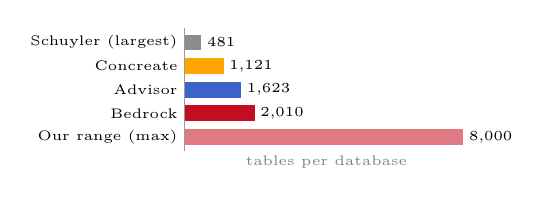
\begin{tikzpicture}[font=\tiny]
  %% tables per database, linear axis 0..8,000 mapped to 0..3.6 cm
  \def\sc{0.00045}
  \foreach \y/\lbl/\n/\nl/\col in {0/Schuyler (largest)/481/{481}/black!45, -0.3/Concreate/1121/{1,121}/color4, -0.6/Advisor/1623/{1,623}/tugb, -0.9/Bedrock/2010/{2,010}/tug, -1.2/Our range (max)/8000/{8,000}/tug!55} {
    \node[anchor=east, inner sep=1pt] at (-0.05,\y) {\lbl};
    \fill[\col] (0,\y-0.1) rectangle (\n*\sc,\y+0.1);
    \node[anchor=west, inner sep=1pt] at (\n*\sc+0.03,\y) {\nl};
  }
  \draw[black!40] (0,0.18) -- (0,-1.38);
  \node[anchor=north, text=gray, inner sep=1pt] at (1.8,-1.4) {tables per database};
\end{tikzpicture}
\end{column}
\begin{column}{0.55\textwidth}
\begin{alertblock}{}
\vspace{0.5mm}
\textbf{Clusters decide which pairs are compared.} In Schuyler's benchmark\rf{2}, only \textbf{60\%} of foreign keys stay inside one cluster:
join only \textbf{within} clusters $\Rightarrow$ lose up to \hred{40\%} of joins;
join \textbf{across} clusters $\Rightarrow$ back to all pairs.
\vspace{0.5mm}
\end{alertblock}
\end{column}
\end{columns}
\end{frame}

%% ─── P1 QUADRATIC COST ───────────────────────────────────────────────────────
\begin{frame}{\apptitle{tug}{Problem 2}{Pairwise Prompting Costs Grow Quadratically}}
\footnotesize
\begin{columns}[T]
\begin{column}{0.55\textwidth}
\centering
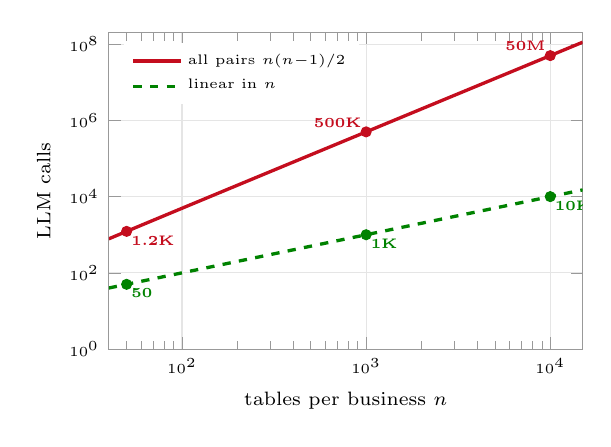
\begin{tikzpicture}
\begin{axis}[
  xmode=log, ymode=log, width=7.6cm, height=5.6cm,
  xmin=40, xmax=15000, ymin=1, ymax=2e8,
  ytick={1,1e2,1e4,1e6,1e8},
  xlabel={tables per business $n$}, ylabel={LLM calls}, label style={font=\scriptsize},
  tick label style={font=\tiny}, axis line style={black!40}, tick style={black!40},
  grid=major, grid style={black!10}, legend style={font=\tiny, draw=none, at={(0.03,0.97)}, anchor=north west}, legend cell align=left]
  \addplot[tug, line width=1.2pt, domain=40:15000, samples=60] {x*(x-1)/2};
  \addplot[darkgreen, line width=1.2pt, dashed, domain=40:15000, samples=60] {x};
  \addplot[only marks, mark=*, mark size=1.8pt, tug] coordinates {(50,1225) (1000,499500) (10000,49995000)};
  \node[font=\tiny\bfseries, anchor=north west, text=tug, inner sep=1.5pt] at (axis cs:50,1225) {1.2K};
  \node[font=\tiny\bfseries, anchor=south east, text=tug, inner sep=1.5pt] at (axis cs:1000,499500) {500K};
  \node[font=\tiny\bfseries, anchor=south east, text=tug, inner sep=1.5pt] at (axis cs:10000,49995000) {50M};
  %% linear reference: one call per table
  \addplot[only marks, mark=*, mark size=1.8pt, darkgreen, forget plot] coordinates {(50,50) (1000,1000) (10000,10000)};
  \node[font=\tiny\bfseries, anchor=north west, text=darkgreen, inner sep=1.5pt] at (axis cs:50,50) {50};
  \node[font=\tiny\bfseries, anchor=north west, text=darkgreen, inner sep=1.5pt] at (axis cs:1000,1000) {1K};
  \node[font=\tiny\bfseries, anchor=north west, text=darkgreen, inner sep=1.5pt] at (axis cs:10000,10000) {10K};
  \legend{all pairs $n(n{-}1)/2$, linear in $n$}
\end{axis}
\end{tikzpicture}
\end{column}
\begin{column}{0.43\textwidth}
\vspace{2mm}
\begin{itemize}\setlength\itemsep{6pt}
  \item Every call carries \textbf{two schemas} and \textbf{sample rows}
  \item 10K tables $\Rightarrow$ \hred{$\approx$50M} calls per business
  \item Almost every call answers \hred{``no join''}
\end{itemize}
\vspace{2mm}
\evidence{Advisor, Bedrock, and Concreate contain 0.6M--2.0M table pairs in the exported subgraph alone.}
\vspace{3mm}
\begin{alertblock}{}
\vspace{0.5mm}
\textbf{Goal:} LLM calls that grow with \textbf{what joins}, not with \textbf{every pair}.
\vspace{0.5mm}
\end{alertblock}
\end{column}
\end{columns}
\end{frame}

%% ─── P2 WRONG JOINS ──────────────────────────────────────────────────────────
\begin{frame}{\apptitle{tug}{Problem 3}{Cheap Signals Produce Wrong Joins --- and Miss Real Ones}}
\footnotesize
\vspace{1mm}
\begin{columns}[T]
\begin{column}{0.49\textwidth}
\textbf{\hred{False joins from accidental overlap}}
\begin{itemize}\setlength\itemsep{3pt}
  \item Surrogate IDs $1..m$ are \textbf{always} contained in $1..n$, $n \geq m$
  \item Status codes, years, and flags overlap everywhere
  \item Street names overlap last names (``Lincoln'', ``Washington'')
\end{itemize}
\evidence{LakeBench\rf{1}: JOSIE\rf{3} ranks the street-name column in the top-$k$ for a last-name query.}\par
\vspace{3mm}
\begin{center}
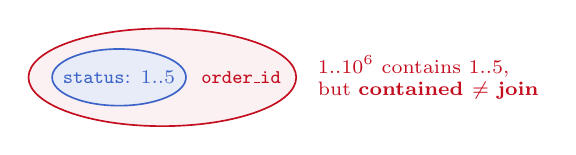
\begin{tikzpicture}[font=\scriptsize]
  \draw[tug, fill=tug!6, line width=0.6pt] (0,0) ellipse (1.7 and 0.62);
  \draw[tugb, fill=tugb!12, line width=0.6pt] (-0.55,0) ellipse (0.85 and 0.36);
  \node[text=tugb] at (-0.55,0) {\texttt{status}: 1..5};
  \node[text=tug] at (1.0,0) {\texttt{order\_id}};
  \node[text=tug, anchor=west, align=left] at (1.85,0) {1..$10^6$ contains 1..5,\\ but \textbf{contained $\neq$ join}};
\end{tikzpicture}
\end{center}
\end{column}
\begin{column}{0.49\textwidth}
\textbf{\hblue{Real joins that look imperfect}}
\begin{itemize}\setlength\itemsep{3pt}
  \item Staging copies keep only recent rows $\Rightarrow$ \textbf{partial} containment
  \item Formats differ (\texttt{00123} vs.\ \texttt{123}, \texttt{P-123}) $\Rightarrow$ \textbf{zero} overlap
  \item One key, many names: \texttt{PROJECT\_CODE}, \texttt{PRJ\_ID}, \texttt{ENGAGEMENT}
\end{itemize}
\evidence{LakeBench\rf{1}: on fuzzy-overlap joins, JOSIE\rf{3} reaches \hred{0\%} top-10 accuracy, DeepJoin\rf{5} \hred{33\%}.}
\vspace{2mm}
\begin{exampleblock}{}
\vspace{0.5mm}
A join needs \textbf{meaning} and \textbf{overlap}. Statistics see overlap; only the LLM sees meaning.
\vspace{0.5mm}
\end{exampleblock}
\end{column}
\end{columns}
\end{frame}

%% ─── P3 REDUNDANCY ───────────────────────────────────────────────────────────
\begin{frame}{\apptitle{tug}{Problem 4}{Redundant Joins Blow Up the Graph}}
\footnotesize
\begin{columns}[T]
\begin{column}{0.50\textwidth}
\centering
\vspace{2mm}
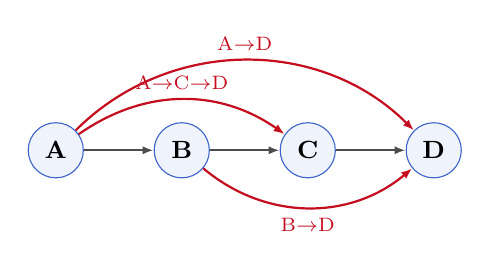
\begin{tikzpicture}[font=\scriptsize, node distance=12mm,
  t/.style={circle, draw=tugb, fill=tugb!8, minimum size=7mm, inner sep=0, font=\small\bfseries},
  e/.style={-{Latex[length=4pt]}, line width=0.8pt}]
  \node[t] (A) at (0,0) {A};
  \node[t] (B) at (1.6,0) {B};
  \node[t] (C) at (3.2,0) {C};
  \node[t] (D) at (4.8,0) {D};
  \draw[e, black!70] (A) -- (B);
  \draw[e, black!70] (B) -- (C);
  \draw[e, black!70] (C) -- (D);
  \draw[e, tug, bend left=35] (A) to node[above, text=tug] {A$\to$C$\to$D} (C);
  \draw[e, tug, bend left=45] (A) to node[above, text=tug] {A$\to$D} (D);
  \draw[e, tug, bend right=40] (B) to node[below, text=tug] {B$\to$D} (D);
\end{tikzpicture}

\vspace{2mm}
{\scriptsize \textcolor{black!70}{\textbf{---}} chain \quad \textcolor{tug}{\textbf{---}} shortcuts already implied by the chain}
\end{column}
\begin{column}{0.48\textwidth}
\vspace{1mm}
\begin{itemize}\setlength\itemsep{5pt}
  \item A key shared by $k$ tables yields $O(k^2)$ pairwise edges
  \item The answers \textbf{follow} from $k$ references to one owner
  \item Queries over the graph must choose among many paths
\end{itemize}
\end{column}
\end{columns}
\vspace{4mm}
\begin{alertblock}{Caution: joins do not always chain}
\vspace{0.5mm}
\texttt{Employee}$\to$\texttt{Dept}$\to$\texttt{Site} is the \emph{office} site, while
\texttt{Employee}$\to$\texttt{Site} may be the \emph{home} site.
A shortcut is redundant \textbf{only if the same key values flow along the path}.
\vspace{0.5mm}
\end{alertblock}
\end{frame}

%% ─── P4 INCONSISTENCY ────────────────────────────────────────────────────────
\begin{frame}{\apptitle{tug}{Problem 5}{Independent Answers Are Inconsistent}}
\footnotesize
\begin{columns}[c]
\begin{column}{0.50\textwidth}
\centering
\begin{tikzpicture}[font=\scriptsize,
  tb/.style={draw=tugb, fill=tugb!5, rounded corners=2pt, line width=0.7pt, inner sep=1.5mm, align=center},
  num/.style={circle, fill=black!70, text=white, inner sep=0.6pt, font=\tiny\bfseries}]
  \node[tb] (P) at (2.1,2.7) {\tikz[baseline=-0.6ex]\pic{tbl=tugb};~\textbf{PROJECT}\\[1pt]\texttt{PROJECT\_CODE} {\tiny(unique)}};
  \node[tb] (T) at (0,0)     {\tikz[baseline=-0.6ex]\pic{tbl=tugb};~\textbf{TIMESHEET}\\[1pt]\texttt{PRJ\_ID}};
  \node[tb] (I) at (4.2,0)   {\tikz[baseline=-0.6ex]\pic{tbl=tugb};~\textbf{INVOICE}\\[1pt]\texttt{ENGAGEMENT}};
  \draw[-{Latex[length=4pt]}, darkgreen, line width=1pt] (T) -- node[left=2pt, align=right, text=darkgreen]
    {\tikz\node[num]{1};~\faCheck\ join} (P);
  \draw[-{Latex[length=4pt]}, darkgreen, line width=1pt] (I) -- node[right=2pt, align=left, text=darkgreen]
    {\tikz\node[num]{2};~\faCheck\ join} (P);
  \draw[tug, line width=1pt, densely dashed] (T) -- node[below=3pt, text=tug]
    {\tikz\node[num]{3};~\faTimes\ ``no join''} (I);
  \node[text=gray, font=\tiny, align=center] at (2.1,-1.05) {one prompt per pair: three separate answers};
\end{tikzpicture}
\end{column}
\begin{column}{0.48\textwidth}
\begin{itemize}\setlength\itemsep{5pt}
  \item Prompts \textbf{1} and \textbf{2}: both columns refer to \texttt{PROJECT\_CODE} \faArrowRight\ \hgreen{join}
  \item Prompt \textbf{3} sees only \texttt{TIMESHEET} and \texttt{INVOICE}: names differ, a few sample rows do not overlap \faArrowRight\ \hred{``no join''}
  \item Together they \textbf{contradict}: two columns with the same key \textbf{do} join through \texttt{PROJECT\_CODE}
  \item The graph shows all three answers, but \textbf{not which one is wrong}
\end{itemize}
\end{column}
\end{columns}
\vspace{4mm}
\begin{exampleblock}{}
\vspace{0.5mm}
\textbf{One ring instead of three pairs:} \texttt{PROJECT\_CODE} $\leftarrow$ \{\texttt{PRJ\_ID}, \texttt{ENGAGEMENT}\} --- one decision, no contradiction.
\vspace{0.5mm}
\end{exampleblock}
\end{frame}

%%%%%%%%%%%%%%%%%%%%%%%%%%%%%%%%%%%%%%%%%%%%%%%%%%%%%%%%%%%%%%%%%%%%%%%%%%%
% \sectionslide{black!60}{EXISTING WORK}  % removed
%%%%%%%%%%%%%%%%%%%%%%%%%%%%%%%%%%%%%%%%%%%%%%%%%%%%%%%%%%%%%%%%%%%%%%%%%%%

%% ─── LANDSCAPE ───────────────────────────────────────────────────────────────
\begin{frame}{\apptitle{black!60}{Existing Work}{Non-LLM, LLM, and Hybrid Join Discovery}}
\scriptsize
\vspace{2mm}
\renewcommand{\arraystretch}{1.3}
\setlength{\tabcolsep}{4pt}
\begin{tabularx}{\textwidth}{@{}>{\raggedright\arraybackslash}p{2.1cm}>{\raggedright\arraybackslash}X>{\raggedright\arraybackslash}X>{\raggedright\arraybackslash}X>{\columncolor{uwmath!7}\raggedright\arraybackslash}X@{}}
\toprule
 & \textbf{Non-LLM}\newline {\tiny IND discovery\rf{10}, Auto-BI\rf{6}, LSH Ensemble\rf{4}, JOSIE\rf{3}, DeepJoin\rf{5}}
 & \textbf{LLM}\newline {\tiny all-pairs prompting}
 & \textbf{Hybrid}\newline {\tiny LOTUS\rf{7}, BARGAIN\rf{8}, FDJ\rf{9}, Schuyler\rf{2}}
 & \textbf{\textcolor{uwmath}{Ours}}\newline {\tiny key domains} \\
\midrule
Decides by meaning & \textcolor{tug}{\ding{55}} overlap \& names & \textcolor{darkgreen}{\ding{51}} & \textcolor{darkgreen}{\ding{51}} if routed to LLM & \textcolor{darkgreen}{\ding{51}} LLM per ring \\
LLM calls grow with & n/a & \textcolor{tug}{\ding{55}} table pairs & \textcolor{tug}{\ding{55}} candidate pairs & \textcolor{darkgreen}{\ding{51}} key domains \\
Recall guarantee & \textcolor{tug}{\ding{55}} & n/a (asks all) & \textcolor{darkgreen}{\ding{51}} per operator & \textcolor{darkgreen}{\ding{51}} vs.\ all-pairs LLM \\
Needs labels & \textcolor{tug}{\ding{55}} (Auto-BI) & \textcolor{darkgreen}{\ding{51}} none & \textcolor{darkgreen}{\ding{51}} none & \textcolor{darkgreen}{\ding{51}} own LLM answers \\
Consistent graph & partly (Auto-BI) & \textcolor{tug}{\ding{55}} independent & \textcolor{tug}{\ding{55}} independent & \textcolor{darkgreen}{\ding{51}} star per key \\
\bottomrule
\end{tabularx}

\vspace{2mm}
\begin{columns}[T]
\begin{column}{0.32\textwidth}\centering
\textbf{\hblue{Non-LLM}}: cheap, but blind to meaning\\{\tiny LakeBench\rf{1}: no method wins everywhere}
\end{column}
\begin{column}{0.32\textwidth}\centering
\textbf{\hred{LLM}}: accurate, but $O(n^2)$\\{\tiny the oracle we want to match}
\end{column}
\begin{column}{0.32\textwidth}\centering
\textbf{\textcolor{uwgoldD}{Hybrid}}: cheaper per pair, still pairwise\\{\tiny BARGAIN\rf{8} defers $\approx$80\% of pairs\rf{9}}
\end{column}
\end{columns}
\end{frame}

%% ─── REFERENCES ──────────────────────────────────────────────────────────────
\newcommand{\refitem}[2]{\item[\textcolor{gray}{[#1]}] #2}
\begin{frame}{\apptitle{black!60}{References}{References}}
\tiny
\vspace{2mm}
\begin{columns}[T]
\begin{column}{0.49\textwidth}
\begin{itemize}\setlength\itemsep{5pt}\setlength\labelwidth{4mm}
  \refitem{1}{Y.~Deng, C.~Chai, L.~Cao, et al. \textbf{LakeBench}: A Benchmark for Discovering Joinable and Unionable Tables in Data Lakes. \emph{PVLDB} 17(8), 2024.}
  \refitem{2}{L.~Laskowski, F.~Panse, M.~Hladik, J.~Portisch, F.~Naumann. \textbf{Schuyler}: Self-Supervised Clustering of Tables in Relational Databases. \emph{PVLDB} 19(4), 2025.}
  \refitem{3}{E.~Zhu, D.~Deng, F.~Nargesian, R.~J.~Miller. \textbf{JOSIE}: Overlap Set Similarity Search for Finding Joinable Tables in Data Lakes. \emph{SIGMOD} 2019.}
  \refitem{4}{E.~Zhu, F.~Nargesian, K.~Q.~Pu, R.~J.~Miller. \textbf{LSH Ensemble}: Internet-Scale Domain Search. \emph{PVLDB} 9(12), 2016.}
  \refitem{5}{Y.~Dong, C.~Xiao, T.~Nozawa, M.~Enomoto, M.~Oyamada. \textbf{DeepJoin}: Joinable Table Discovery with Pre-trained Language Models. \emph{PVLDB} 16(10), 2023.}
\end{itemize}
\end{column}
\begin{column}{0.49\textwidth}
\begin{itemize}\setlength\itemsep{5pt}\setlength\labelwidth{4mm}
  \refitem{6}{Y.~Lin, Y.~He, S.~Chaudhuri. \textbf{Auto-BI}: Automatically Build BI-Models Leveraging Local Join Prediction and Global Schema Graph Optimization. \emph{PVLDB} 16(10), 2023.}
  \refitem{7}{L.~Patel, S.~Jha, C.~Guestrin, M.~Zaharia. \textbf{LOTUS}: Enabling Semantic Queries with LLMs Over Tables of Unstructured and Structured Data. \emph{arXiv:2407.11418}, 2024.}
  \refitem{8}{S.~Zeighami, S.~Shankar, A.~Parameswaran. Cut Costs, Not Accuracy: LLM-Powered Data Processing with Guarantees (\textbf{BARGAIN}). \emph{SIGMOD} 2026.}
  \refitem{9}{S.~Zeighami, S.~Shankar, A.~Parameswaran. \textbf{Featurized-Decomposition Join}: Low-Cost Semantic Joins with Guarantees. \emph{arXiv:2512.05399}, 2025.}
  \refitem{10}{F.~Tschirschnitz, T.~Papenbrock, F.~Naumann. Detecting \textbf{Inclusion Dependencies} on Very Many Tables. \emph{ACM TODS} 42(3), 2017.}
\end{itemize}
\end{column}
\end{columns}
\end{frame}

%% ═══ hidden for now: everything after Existing Work (remove \iffalse/\fi to show again) ═══
\iffalse

%%%%%%%%%%%%%%%%%%%%%%%%%%%%%%%%%%%%%%%%%%%%%%%%%%%%%%%%%%%%%%%%%%%%%%%%%%%
\sectionslide{uwmath}{RESEARCH PROBLEM}
%%%%%%%%%%%%%%%%%%%%%%%%%%%%%%%%%%%%%%%%%%%%%%%%%%%%%%%%%%%%%%%%%%%%%%%%%%%

%% ─── PROBLEM DEFINITION ──────────────────────────────────────────────────────
\begin{frame}{\apptitle{uwmath}{Research Problem}{Cost-Bounded Join Key Discovery}}
\footnotesize
\vspace{1mm}
\begin{block}{Problem}
\vspace{1mm}
Given a database $\mathcal{D}$ with tables $T_1,\dots,T_n$ and \textbf{no declared keys}, an LLM oracle $\mathcal{O}$,
a recall target $\gamma$, and a confidence $1-\delta$, find the join set $\hat{J}$ that
\[
\min\ \mathrm{cost}_{\mathrm{LLM}}
\qquad \text{s.t.} \qquad
\Pr\big[\,|\hat{J} \cap J^*| \,/\, |J^*| \;\geq\; \gamma\,\big] \;\geq\; 1-\delta
\]
where $J^*$ is the join set of \textbf{all-pairs prompting} ($n(n{-}1)/2$ oracle calls).
\vspace{1mm}
\end{block}
\vspace{2mm}
\begin{columns}[T]
\begin{column}{0.49\textwidth}
\begin{itemize}\setlength\itemsep{4pt}
  \item[\textcolor{uwmath}{\textbf{R1}}] \textbf{Recall-guaranteed} --- keep $\geq\gamma$ of the oracle's joins w.p.\ $\geq 1-\delta$
  \item[\textcolor{uwmath}{\textbf{R2}}] \textbf{Domain-proportional} --- LLM calls grow with key domains, not pairs
\end{itemize}
\end{column}
\begin{column}{0.49\textwidth}
\begin{itemize}\setlength\itemsep{4pt}
  \item[\textcolor{uwmath}{\textbf{R3}}] \textbf{Label-free} --- learn only from the LLM answers we pay for
  \item[\textcolor{uwmath}{\textbf{R4}}] \textbf{Consistent} --- every reference points to one owner; no redundant edges
\end{itemize}
\end{column}
\end{columns}
\end{frame}

%% ─── KEY INSIGHT ─────────────────────────────────────────────────────────────
\begin{frame}{\apptitle{uwmath}{Key Insight}{Label Key Domains, Not Table Pairs}}
\footnotesize
\begin{columns}[c]
\begin{column}{0.46\textwidth}
\begin{itemize}\setlength\itemsep{6pt}
  \item Joins concentrate on a few \hring{key domains}: customer, project, employee, invoice IDs
  \item Each domain has one unique \textbf{owner} and many \textbf{member} columns
  \item Know the domains $\Rightarrow$ know the joins: every member joins its owner
  \item \#domains $\ll$ \#table pairs
\end{itemize}
\vspace{3mm}
\begin{exampleblock}{}
\vspace{0.5mm}
Work \textbf{linear in columns} (profiling, grouping) replaces work \textbf{quadratic in tables} --- FDJ's insight, lifted from records to schemas.
\vspace{0.5mm}
\end{exampleblock}
\end{column}
\begin{column}{0.52\textwidth}
\centering
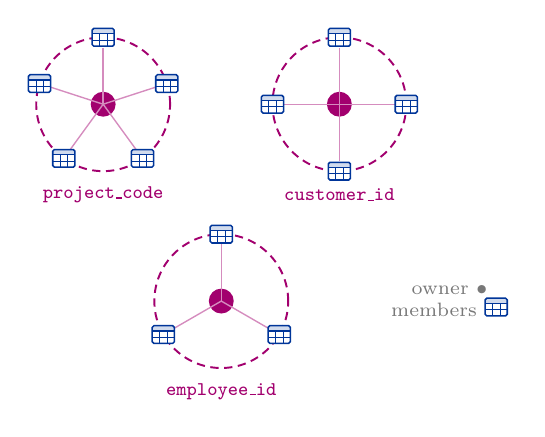
\begin{tikzpicture}[font=\scriptsize]
  \foreach \cx/\nm/\lbl/\k in {0/R1/project\_code/5, 3.0/R2/customer\_id/4, 1.5/R3/employee\_id/3} {
    \pgfmathsetmacro{\cy}{ifthenelse(\cx==1.5,-2.5,0)}
    \draw[uwmath, densely dashed, line width=0.7pt] (\cx,\cy) circle (0.85);
    \node[circle, fill=uwmath, minimum size=9pt, inner sep=0] at (\cx,\cy) {};
    \foreach \i in {1,...,\k} {
      \draw[uwmath!45, line width=0.5pt] (\cx,\cy) -- ($(\cx,\cy)+({90+360*\i/\k}:0.72)$);
      \pic[scale=0.8] at ($(\cx,\cy)+({90+360*\i/\k}:0.85)$) {tbl=uwsci};
    }
    \node[text=uwmath, font=\scriptsize\ttfamily] at (\cx,\cy-1.15) {\lbl};
  }
  \node[align=center, text=uwgreyC] at (4.4,-2.5) {owner $\bullet$\\members \tikz\pic[scale=0.8]{tbl=uwsci};};
\end{tikzpicture}
\end{column}
\end{columns}
\end{frame}

%%%%%%%%%%%%%%%%%%%%%%%%%%%%%%%%%%%%%%%%%%%%%%%%%%%%%%%%%%%%%%%%%%%%%%%%%%%
\sectionslide{darkgreen}{KEYRING}
%%%%%%%%%%%%%%%%%%%%%%%%%%%%%%%%%%%%%%%%%%%%%%%%%%%%%%%%%%%%%%%%%%%%%%%%%%%

%% ─── ARCHITECTURE ────────────────────────────────────────────────────────────
\begin{frame}{\apptitle{darkgreen}{KeyRing}{System Architecture}}
\footnotesize
\vspace{1mm}
\centering
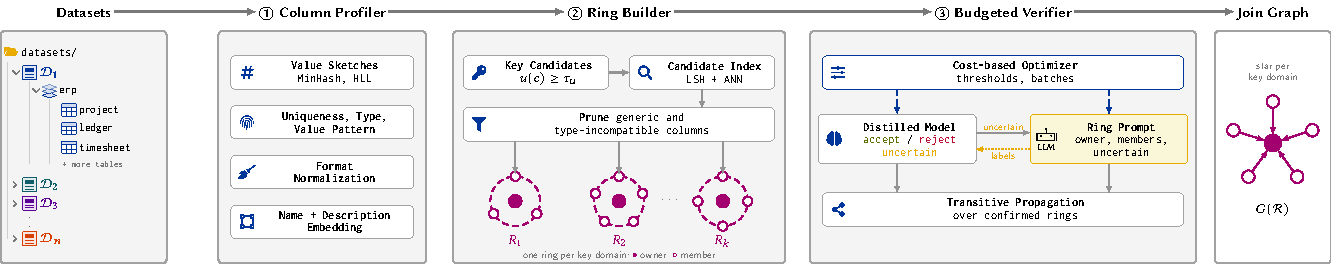
\includegraphics[width=\textwidth]{fig/fig_KeyRing_Architecture.pdf}

\vspace{3mm}
\begin{columns}[T]
\begin{column}{0.32\textwidth}
\textbf{\textcircled{\scriptsize 1} Column Profiler}\\
one pass, \hgreen{no LLM}: sketches, uniqueness, normalized formats, embeddings
\end{column}
\begin{column}{0.32\textwidth}
\textbf{\textcircled{\scriptsize 2} Ring Builder}\\
candidate keys $\to$ indexes $\to$ prune generic columns $\to$ \hring{rings} with owners
\end{column}
\begin{column}{0.32\textwidth}
\textbf{\textcircled{\scriptsize 3} Budgeted Verifier}\\
distilled model decides confident cases; \textbf{one LLM prompt per ring}; recall $\geq\gamma$
\end{column}
\end{columns}
\end{frame}

%% ─── RESEARCH QUESTIONS ──────────────────────────────────────────────────────
\begin{frame}{\apptitle{darkgreen}{Research Agenda}{Research Questions}}
\footnotesize
\vspace{2mm}
\begin{columns}[T]
\begin{column}{0.49\textwidth}
\begin{block}{Paper 1 --- Cost (KeyRing)}
\vspace{1mm}
\begin{itemize}\setlength\itemsep{4pt}
  \item[\textbf{RQ1}] How do we discover \textbf{key domains} and elect owners at scale without the LLM?
  \item[\textbf{RQ2}] How do we route candidates to keep \textbf{recall $\geq\gamma$} with the fewest LLM calls?
  \item[\textbf{RQ3}] Can a \textbf{distilled local model} replace the LLM for most candidates, and transfer across businesses?
\end{itemize}
\vspace{1mm}
\end{block}
\end{column}
\begin{column}{0.49\textwidth}
\begin{block}{Paper 2 --- Quality}
\vspace{1mm}
\begin{itemize}\setlength\itemsep{4pt}
  \item[\textbf{RQ4}] What is a \textbf{minimal equivalent join graph} when joins do not always chain?
  \item[\textbf{RQ5}] Can \textbf{cycle consistency} expose wrong joins that look fine pair by pair?
  \item[\textbf{RQ6}] How do we separate \textbf{union} (snapshots, versions) from \textbf{join}?
\end{itemize}
\vspace{1mm}
\end{block}
\end{column}
\end{columns}
\end{frame}

%% ─── EVALUATION PLAN ─────────────────────────────────────────────────────────
\begin{frame}{\apptitle{darkgreen}{Research Agenda}{Evaluation Plan}}
\footnotesize
\vspace{2mm}
\begin{columns}[T]
\begin{column}{0.32\textwidth}
\textbf{\hblue{Data}}
\begin{itemize}\setlength\itemsep{3pt}
  \item Production databases of several businesses (50--10K tables)
  \item Existing all-pairs LLM results as the \textbf{oracle} and as free labels
  \item Human-labeled sample for absolute precision and recall
\end{itemize}
\end{column}
\begin{column}{0.32\textwidth}
\textbf{\hred{Baselines}}
\begin{itemize}\setlength\itemsep{3pt}
  \item \textbf{Non-LLM}: IND discovery, Auto-BI, JOSIE / LSH Ensemble, DeepJoin
  \item \textbf{LLM}: all-pairs prompting
  \item \textbf{Hybrid}: LOTUS / BARGAIN cascades, FDJ
\end{itemize}
\end{column}
\begin{column}{0.32\textwidth}
\textbf{\hgreen{Metrics}}
\begin{itemize}\setlength\itemsep{3pt}
  \item LLM calls, tokens, \$, end-to-end time
  \item Recall vs.\ oracle at target $\gamma$; precision; F1
  \item Graph size: edges per table, redundant edges
\end{itemize}
\end{column}
\end{columns}

\vspace{5mm}
\begin{exampleblock}{}
\vspace{0.5mm}
\centering
\textbf{Headline to show:} \hgreen{orders of magnitude fewer LLM calls} than all-pairs prompting at \textbf{the same recall}, and \hgreen{higher F1} than the best non-LLM method.
\vspace{0.5mm}
\end{exampleblock}
\end{frame}

%% ─── SUMMARY ─────────────────────────────────────────────────────────────────
\begin{frame}{\apptitle{black!60}{Summary}{Takeaways}}
\footnotesize
\vspace{3mm}
\begin{enumerate}\setlength\itemsep{8pt}
  \item \textbf{Today's join graphs are dense and untrustworthy}: hubs on generic columns, snapshot cliques, hundreds of edges per table.
  \item \textbf{All-pairs prompting is the right oracle but the wrong algorithm}: $O(n^2)$ calls, mostly ``no join''.
  \item \textbf{Non-LLM and hybrid methods do not close the gap}: blind to meaning, or still pairwise.
  \item \textbf{KeyRing labels key domains, not pairs}: LLM calls grow with domains, recall is guaranteed, and the graph is a star per key.
\end{enumerate}
\vspace{4mm}
\begin{block}{Next steps}
\vspace{1mm}
Export full edge lists \faAngleRight\ profile all columns \faAngleRight\ measure candidate recall \faAngleRight\ prototype rings \faAngleRight\ cost/recall experiments
\vspace{1mm}
\end{block}
\end{frame}

\fi

\end{document}
